\documentclass[a4paper,12pt]{article} % тип документа

% report, book



%  Русский язык

\usepackage[T2A]{fontenc}			% кодировка
\usepackage[utf8]{inputenc}			% кодировка исходного текста
\usepackage[english,russian]{babel}	% локализация и переносы
\usepackage{graphicx}
\graphicspath{{./}}
\DeclareGraphicsExtensions{.png,.jpg}


% Математика
\usepackage{amsmath,amsfonts,amssymb,amsthm,mathtools} 


\usepackage{wasysym}

%Заговолок
\author{Бредихин Александр}
\title{Домашняя работа №5}



\begin{document} % начало документа

\maketitle

\subsection*{Задача 1}
Задача: дан массив длины $n$, состоящий только из нулей и единиц. Предложите линейный алгоритм сортировки данного массива.\\

Сортировка подсчётом: так как элементами в массиве могут быть только $ 0 $ или $ 1 $, то заведём два счётчика: $ count\_0  $, $ count\_1 $. Идём по входному массиву, если встречаем 0, то $ count\_0 ++ $ иначе $ count\_1 ++$. Затем выводим сначала $ count\_0 $ нулей, затем $ count\_1 $ единиц, получаем отсортированный массив.\\
Корректность: выведенный массив отсортирован, так как все единицы идут после нулей и количество нулей в исходном и в выведеном совпадает (на каждом шаге по исходному массиву инкрементируется одна из переменных).\\ Сложность алгоритма: $ O(n) $ (проходим один раз по массиву длинной $ n $ и затем печатаем $ n $ чисел).


\subsection*{Задача 2}
Задача: на прямой задано $n$ отрезков, причем известно, что они образуют систему строго вложенных отрезков (их можно упорядочить так, чтобы каждый строго содержался в следующем). Отрезки заданы координатами концов $[l_i, r_i]$ (и могут быть даны в неупорядоченном виде). Предложите асимптотически эффективный алгоритм (с точки зрения количества арифметических операций), который находит все точки прямой, которые покрыты ровно $2n/3$ отрезками.\\

Заметим, что если бы массив был отсортирован по левым границам (все отрезки вложены, поэтому правые границы тоже останутся отсортированными и не будет пересечения отрезков), то искомые точки расположены между двумя левыми концами с номерами $ \frac{2n}{3} $ и $ \frac{2n}{3}+1 $ и их же правыми концами (нумерация отрезков происходит от самого короткого к самому длинному по длине отрезка) (как раз берём все точки, которые покрыты ровно  $2n/3$ отрезками).\\

Алгоритм: с помощью алгоритма по нахождению $ k $ой порядковой статистики ищем $ \frac{2n}{3} $ и $ \frac{2n}{3}+1 $ порядковые статистики в исходном массиве левых границ. Пусть элемент $ l_1 = \frac{2n}{3} $ порядковой статичстики, $ l_2 = \frac{2n}{3} $ -- правой. $ r_1 $ и $ r_2 $ соответсвующие правые границы, тогда ответом на задачу будут точки удволетворяющие:  $ x \in\left[l_{1}, l_{2}\right] \cup\left[r_{1}, r_{2}\right] $ (корректность ответа обоснована выше).\\

Сложность: алгоритм нахождения $ k $ой порядковой статистики работает за $ \mathcal{O}(n) $, где $ n $ -- количество отрезков (правых и левых границ). Мы вызываем этот алгоритм 2 раза, следовательно сложность нашей задачи $ \mathcal{O}(n)  $.



\subsection*{Задача 3}
Задача: рассмотрим детерминированный алгоритм поиска порядковой статистики за линейное время из параграфа 9.3 Кормена. Какая асимптотика будет у алгоритма, если делить элементы массива на группы по семь, а не по пять?\\

Из семинара, оценка работы алгоритма в общем случае:\\
будем рассматривать входной массив размером $ n $ и разбивать его на $ 2k+1 $ элементные группы. Внутри каждой группы сортируем элементы и берём медиану каждой группы и из них ищем медиану медиан $ m^* $ рекурсивно. Количество групп в которых медианы меньше $ m^* $ оценивается как $ \frac{n}{2(2k+1)} $, следовательно, количество элементов в исходном ммассиве меньших $ m^* $ оценивается $ \frac{n}{2(2k+1)} \cdot (k+1) $. Получается, левее медианы медиан стоит как минимум $ \frac{n(k+1)}{2(2k+1)} $, а правее не более                $ n - \frac{n(k+1)}{2(2k+1)} = \frac{n(3k+1)}{4k+2} $. Затем запускаемся от каждой из этих частей. Рекурентная формула:
$$
T(n)=c n+T\left(\frac{n}{2 k+1}\right)+T\left(\frac{n(3 k+1)}{4 k+2}\right)
$$
для $ k = 3 $ она имеет вид:
$$
T(n)=c n+T\left(\frac{n}{7}\right)+T\left(\frac{5 n}{7}\right)
$$
Разрешим эту рекуренту с помощью дерева вызовов:
\begin{center}
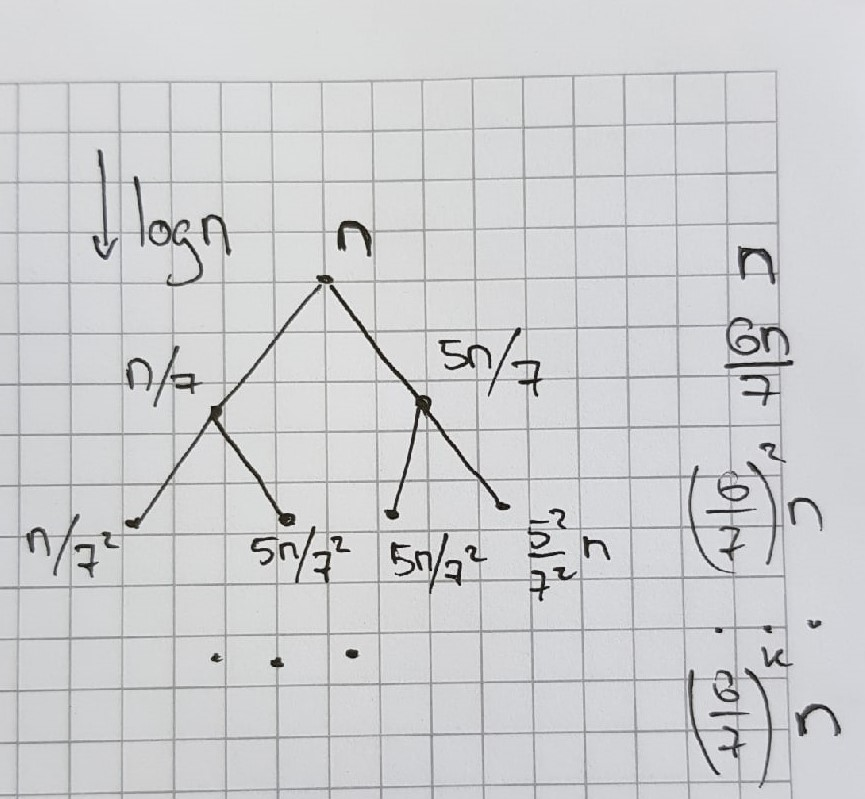
\includegraphics[width=0.7\textwidth]{tree_3}
\end{center}
Заметим, что в каждой строчке сумма операций равна: $ \left( \frac{6}{7} \right)^k \cdot n $ (бином Ньютона). Тогда всего количество операций: $ \sum\limits_{k=0}^{\log n}\left(\frac{6}{7}\right)^{k} \cdot n=7 \cdot n \cdot\left(1-\left(\frac{6}{7}\right)^{\log n}\right) $
При больших $ n $ получаем: $ T(n) = \Theta(n) $\\
Ответ: $ \Theta(n) $

\subsection*{Задача 4}
Задача: на вход задачи подаётся число $n$ и массив чисел $x_1, x_2, \ldots, x_{2n+1}$. Постройте линейный алгоритм, находящий число $s$, при котором достигается минимум суммы $$ \sum\limits_{i=1}^{2n+1}|x_i - s|. $$

Ответом на эту задачу, то есть числом $ s $ будет являться медиана массива (так как количество элементов -- нечётное, то  слева и справа от неё лежит одинаковое количество элементов, $ n $), докажем это:\\
функция, данная в задаче определена на $\mathcal{R} $ и принадлечит классу дифференцируемых функций. Нам нужно найти её экстремум (минимум), что соответсвует 0 производной.\\
Производная функции: $ \sum\limits_{i=1}^{2n+1}sign(x_i - s) $. Это функция равна 0, тогда и только тогда, когда $ s = x_{n+1} $ (количество $+1  $ равно числу $ -1 $). Докажем, что это значение соответсвует минимуму, а не максимуму. Немного сместимся от этой точки б.о.о вправо. Обозначим это число $ a $ (так как мы смещаемся немного, то берём $a$ такое что $ x_{n+1} < a < x_{n+2} $). Обозначим за $ d = a - x_{n+1} $ - смещение.\\
Расстояние между $ x_{n+1} $ и  $ x_{n+2} $ до $ a $ не изменилось. Правее лежит $ n - 1 $ число и расстояние до них уменьшилось на $ d \cdot (n - 1) $, а левее, $ n $ чисел, следовательно расстояние увеличилось на $ d \cdot n $. В итоге функция увеличивается на $ d  $, аналогично, если будем смещаться влево от медианы. Получается, медиана массива -- нужное число $ s $.\\

Алгоритм: применяем алгоритм нахождения медианы масива (выводили на лекции нахождение $ n+1 $ (в этом случае) порядковой статистики). Время работы $ \mathcal{O}(n) $.

\subsection*{Задача 5}
Задача:  предложите полиномиальный от длины входа алгоритм решения сравнения $a\cdot x + b\equiv 0\pmod M$ (На вход дают целые числа $a,b,M$ в двоичной системе исчисления).

Это сравнение эквивалентно такому уравнению в целых числах:
$$
ax + My = -b
$$
К нему можем применить бинарный алгоритм Евклида основанный на фактах:
\begin{itemize}
\item НОД(0, n) = n; НОД(m, 0) = m; НОД(m, m) = m;
\item НОД(1, n) = 1; НОД(m, 1) = 1;
\item Если m, n чётные, то НОД(m, n) = 2*НОД(m/2, n/2);
\item Если m чётное, n нечётное, то НОД(m, n) = НОД(m/2, n);
\item Если n чётное, m нечётное, то НОД(m, n) = НОД(m, n/2);
\item Если m, n нечётные и n > m, то НОД(m, n) = НОД((n-m)/2, m);
\item Если m, n нечётные и n < m, то НОД(m, n) = НОД((m-n)/2, n);
\end{itemize}
Сам алгоритм полностью аналогичен обычному и его сложность $ \mathcal{O}(n^2)$, где $ n $ -- длина максимального из чисел в двоичной записи.

\subsection*{Задача 6}
Задача: 1) оцените глубину стека (рекурсивных вызовов) при работе быстрой сортировки в худшем случае.\\
2) измените алгоритм быстрой сортировки так, чтобы глубина стека в худшем случае была $\Theta(\log n)$\\

1) Подадим функции $ QuickSort $ уже отсортированный массив. Б.о.о. она будет выбирать самый минимальный элемент элемент за опорный (массив будет отсортирован в обратном порядке и за опорный элемент будем брать последний) и перетаскивать его на 1ое место. Тогда следующий вызов будет происходить от части из одного элемента (левая часть) и всех остальных $ n - 1 $ элементов. На следующим шаге аналогичная ситуация и справа остаётся $ n - 2 $ элемента. Получается, мы сделаем $ n $ вложенных рекурсивных вызовов при каждом из которых мы кладём в стек информацию о регистрах и текущем положении (константа по памяти), следовательно, в стек мы будем класть $ \mathcal{O}(n) $ данных в худшем случае, то есть глубина стека линейная.\\
Ответ: $ \mathcal{O}(n) $\\

2) Чтобы не возникало линейного роста глубины стека, нужно, чтобы дерево вызовов было симметрично (то есть каждый раз массив делился на 2 равные части и следующие вызовы были от массива в 2 раза меньшей длины), тогда глубина дерева $ \log n $ -- глубина рекурсии.\\
Как разбивать массив на каждом шаге пополам? Для этого можно на каждом шаге считать $ n/2 $ порядковую статистику (медиану текущего массива) и за опорный элемент брать её, тогда по определению слева и справа от неё будет одинаковое количество элементов (или с различием на 1). 

\subsection*{Задача 7}
Задача: дан массив из $n$ чисел. Нужно разбить этот массив на максимальное количество непрерывных подмассивов так, чтобы после сортировки элементов внутри каждого подмассива весь массив стал отсортированным. Предложите $O(n\log n)$ алгоритм для решения этой задачи.\\

Алгоритм: cначала сортируем исходный массив и делаем замену: первый элемент в отсортированном массиве равняется 1, второй -- 2 и так далее. Возвращаемся к первоначальному расположению элементов в массиве, но уже заменённых своим порядковым номером в отсортированном массиве (по сути своей порядковой статистикой).\\
Нужно разбить получившийся массив на максимальное количество непрерывных подмассивов так, чтобы после сортировки элементов внутри каждого подмассива весь массив стал отсортированным, для этого с первого элемента идём по массиву и на каждом шаге сравниваем номер считанного числа с текущим максимумом, если они на каком-то шаге равны, то отделяем этот массив и продолжаем пока не дойдём до конца.\\

Корректность: если на каком-то моменте максимум равен $ k $ - номеру считанного числа, то мы можем отсортировать полученный подмассив так, чтобы они были упорядоченными по возрастанию и не превышали $k$ и шли подряд, значит этот подмассив можно отрезать (так как его можно отсортировать по возрастанию, чтобы элементы в нём шли подряд).\\
Число полученных таким образом подмассивов максимально, так как если мы возьмём подмассив меньшего размера, то после сортировки где-то в другом подмассиве найдётся элемент, который меньше, чем максимальный в подмассиве ранее (не получится отсортировать весь массив).\\

Сложность: сортировка массива происходит за $\mathcal{O}(n \cdot \log n)$. Дальнейшее разбиение на подмассивы происходит за $ \mathcal{O}(n) $, следовательно, общая сложность занимает $\mathcal{O}(n \cdot \log n)$.

\end{document} % конец документа